\documentclass[useAMS,usenatbib,twocolumn]{mn2e}

%\addtolength{\marginparwidth}{1.875in}

\usepackage{graphicx}
\usepackage{dcolumn}
\usepackage{bm}
\usepackage{listings}
\usepackage{amssymb}
\usepackage{verbatim}
\usepackage{url}
% \usepackage{amsthm}
\usepackage{mathtools}
\usepackage{amsmath}
\usepackage{longtable}
\usepackage{booktabs}
\usepackage{ctable}
% \usepackage{natbib}
% \bibliographystyle{apj}

% Symbol
\makeatletter
\newcommand{\HI}{{\rm H\,{\scriptstyle I}}}
\newcommand{\HII}{{\rm H\,{\scriptstyle II}}}
\newcommand{\HeI}{{\rm He\,{\scriptstyle I}}}
\newcommand{\HeII}{{\rm He\,{\scriptstyle II}}}
\newcommand{\HeIII}{{\rm He\,{\scriptstyle III}}}
\newcommand{\rmnum}[1]{\romannumeral #1}
\newcommand{\Rmnum}[1]{\expandafter\@slowromancap\romannumeral #1@}
\newcommand{\nHI}{n_{\mbox{\tiny H\Rmnum{1}}}}
\newcommand{\xHI}{x_{\mbox{\tiny H\Rmnum{1}}}}
\newcommand{\xHII}{x_{\mbox{\tiny H\Rmnum{2}}}}
\newcommand{\eHI}{\epsilon_{\mbox{\tiny H\Rmnum{1}}}}
\newcommand{\LyA}{\mbox{Ly}\alpha}
\newcommand{\fHI}{\langle f_{\mbox{\tiny H\Rmnum{1}}}\rangle}
\newcommand{\fHII}{\langle f_{\mbox{\tiny H\Rmnum{2}}}\rangle}
\newcommand{\NHI}{N_{\mbox{\tiny H\Rmnum{1}}}}
\newcommand{\NHIi}{N_{\mbox{\tiny H\Rmnum{1}},i}}
\makeatother

%Journals
\newcommand{\aap}{A\&Ap}
\newcommand{\aj}{AJ}
\newcommand{\apj}{ApJ}
\newcommand{\apjl}{ApJ}
\newcommand{\apjs}{ApJS}
\newcommand{\araa}{ARA\&A}
\newcommand{\mnras}{MNRAS}
\newcommand{\physrep}{Phys. Rep.}
\newcommand{\nat}{Nature}


\title[$\LyA$ forests and $\LyA$ galaxy surveys]
  {Joint analysis of galaxy redshift surveys and $\LyA$ forests \Rmnum{1}: \newline
  the large-scale gasenous environment of $\LyA$ galaxies 
  with redshift-space distortion}


\author[K. Kakiichi et al.]
{Koki Kakiichi et al,$^{1}$\thanks{E-mail: kakiichi@mpa-garching.mpg.de}
\\
$^1$Max Planck Institute for Astrophysics, Karl-Schwarzschild Stra\ss e 1, 85741 Garching, Germany
}


\date{Released 2002 Xxxxx XX}

\pagerange{\pageref{firstpage}--\pageref{lastpage}} \pubyear{2002}

\def\LaTeX{L\kern-.36em\raise.3ex\hbox{a}\kern-.15em
    T\kern-.1667em\lower.7ex\hbox{E}\kern-.125emX}

\begin{document}

\maketitle

\begin{abstract}
Redshift surveys of $\LyA$ forests and $\LyA$-emitting/absorbing galaxies. 
\end{abstract}

\begin{keywords}
atomic processes -- cosmology:\ theory -- line:\ formation -- radiative
transfer -- infrared:\ general -- scattering
\end{keywords}

\section{Introduction}
We propose and the explore the potentials of deep redshift surveys
of $\LyA$ galaxies in the foregound of QSOs covering redshifts $2<z<8$.
Joint analysis of $\LyA$ forests and $\LyA$-emitting and absorbing galaxies
over redshift $3<z<8$ enables us to investigate the Epoch of Reionization
and the transition to post-reionization era, allowing to break the multiple 
degeneracies arising from analysis of high-redshift $\LyA$ galaxies alone.
For both Lyman-break and narrow-band selection technique, $\LyA$ line can 
appear in galaxies both as emission or absorption.

The gasenous environment of galaxies is a natural consequence arising from 
the concordance hierarchical structure formation in $\rm{\Lambda CDM}$
cosmology, forming cosmic web. One effect of gasenous environment on
galaxies is the impact on their formation and evolution (Dekel+),
for example, the popular cold stream picture in the formation of galaxies 
to name a few. Another important impact of the environment is to induce
the selection bias on the observation of galaxies. Since we see galaxies
through their gasenous environments, any absorption or reprocessing of the light
along a line of sight introduces the environmentally-induced selection bias 
upon observations of galaxies. One notable example of such selection bias is 
on the population of $\LyA$-emitting galaxies, which has been used to 
constrain the neutral fraction of the universe during the EoR. 
Furthermore, even at the post-reionized universe, the possibile impact 
on LAEs clustering due to the $\LyA$ RT through the gasenous environment 
as CGM and IGM (Zheng+; Wyithe \& Dijkstra; Breg+) calls for the close 
examination and testing this hypothesis based on observations. The degree of 
the environmetal impact on the LAE selection influences the interprelation of 
redshift BAO survey such as HETDEX to do cosmology (Wyithe\&Dijkstra, Breg+). 
 
The galaxy redshift survey in the foreground of QSOs is not a new
idea, which has been conducted by Aldelberger+, Cooke+, Keck Baryonic
Structure Survey (KBSS, Steidel+) for $z\sim2-3$. Yet, the connection
to EoR and RT studies of galaxies and the IGM are not or only weakly made.
The idea to perform the joint analysis of $\LyA$ galaxies and QSO spectra
occasionally has appeared in the literature (Baek, Ferrara \& Semelin 2012,
SDSS J1335+3533 good candidate?). Yet, the full potential of such survey
strategy and the requirement still must be worked out.
An idea is to extend such survey strategy to higher redshifts, which
enable us the joint analysis of LLS/DLA, $\LyA$ forests and galaxies for
both $\LyA$ in emission and absorption.


\section{Survey Requirements}
We propose the sketch of survey requirement to characterise the IGM/CGM 
environment of $\LyA$-galaxies for $2<z<8$.

\subsection{QSO fields}
\begin{table}
\centering
\caption{List of potential targets of QSO fields. QSOs used in Fan+2006 and 
Becker+2014 are listed.} \label{table:qso_field}
\begin{tabular}{lll}
\hline
QSO name                               & QSO redshift  &         \\ 

\hline
$z>6$            &      \\
SDSS J1148+5251                   &  6.4189       & Fan+06  \\
SDSS J1030+0524                   &  6.3110       & Fan+06  \\
CFHQS J0050+3445                  & 6.25 \\
SDSS J1623+3112                   &  6.2470       & Fan+06  \\
SDSS J1048+4637                   &  6.2284       & Fan+06  \\
SDSS J125051.93+313021.9          &  6.1300       & Fan+06  \\
ULAS J1319+0950                   & 6.13 \\
SDSS J2315−0023                   & 6.12 \\
SDSS J1602+4228                   &  6.0700       & Fan+06  \\
SDSS J1630+4012                   &  6.0650       & Fan+06  \\
SDSS J2054−0005                   & 6.06 \\
SDSS J0353+0104                   & 6.05 \\
SDSS J0818+1722                   & 6.02         & Fan+06  \\
SDSS J1306+0356                   &  6.0160       & Fan+06  \\
SDSS J113717.73+354956.9          &  6.0100       & Fan+06  \\
\\
$5<z<6$ \\
ULAS J0148+0600                   & 5.98 \\
SDSS J1411+1217                   &  5.9270       & Fan+06  \\
SDSS J133550.80+353315.8          &  5.9012       & Fan+06  \\
SDSS J0005-0006                   &  5.85         & Fan+06  \\    
SDSS J0840+5624                   &  5.8441       & Fan+06  \\
SDSS J143611.74+500706.9          &  5.8300       & Fan+06  \\
SDSS J104433.04-012502.2          &  5.7824       & Fan+06  \\
SDSS J0836+0054                   &  5.774        & Fan+06  \\
SDSS J092721.82+200123.7          &  5.7722       & Fan+06  \\
SDSS J0203+0012  & 5.72 \\
SDSS J0231−0728  & 5.42 \\ 
SDSS J1659+2709  & 5.32 \\
SDSS J1208+0010  & 5.27 \\
SDSS J0915+4244  & 5.20 \\
SDSS J1204−0021  & 5.09 \\
\\
$4<z<5$ \\
SDSS J0040−0915  & 4.98\\
SDSS J0011+1446  & 4.95\\
SDSS J2225−0014  & 4.89\\
SDSS J1616+0501  & 4.88\\
BR 1202−0725     & 4.70\\
SDSS J2147−0838  & 4.60\\
BR 0353−3820     & 4.59\\
BR 1033−0327     & 4.52\\
BR 0006−6208     & 4.52\\
BR 0714−6449     & 4.49\\
BR 0418−5723     & 4.48\\
\\
$z<3-4$ \\
see BOSS $\LyA$ survey & & Kee-Gee?+ \\
  \hline
\end{tabular}

\end{table}

Firstly, the selection of the potential target fields is listed in
Table $\ref{table:qso_field}$. The redshift range covered by the $\LyA$ 
forest between $\LyA$ and $\mbox{Ly}\beta$ lines in the restframe of a 
background QSO at redshift $z_Q$ is $\Delta z/(1+z_Q)=\Delta\lambda/
\lambda_\alpha$ where $\Delta\lambda=\lambda_\alpha-\lambda_\beta$ is the 
wavelength interval between $\LyA$ and $\mbox{Ly}\beta$ lines.

To perform the Voigt profile decomposition of $\LyA$ forests, both high 
signal-to-noise ratio per pixel and high resolution ($\rm{FWHM\lesssim25km/s}$)
spectroscopy of a QSO should be obtained (\citealt{1998ARA&A..36..267R}). 
For example, KBSS survey (\citealt{2012ApJ...750...67R}) has observed 
15 QSOs with Keck/HIRES, obtaining $R\simeq45000$ 
(FWHM$\simeq 7$km/s) and $\rm{S/N\sim50-200pixel^{-1}}$. The resolved FWHM sets 
the lower limit of $b$-parameter can be measured from voigt profile 
decomposition. 

While the high resolution and high S/N spectroscopy is always desirable 
whenever available, there are a couple of ways to characterise the absorbing 
systems with the equivalent width and redshift using intermediate resolution 
spectroscopy (\citealt{1998ARA&A..36..267R}). We explore the pixel optical 
depth method, EW-redshift indentification, and voigt profile decomposition 
to characterise the CGM/IGM environment using the synthetic spectra from 
simulations in the subsequent section. 


\subsection{Galaxy fields}
\begin{table*}
\centering
\caption{Telescopes and intruments for redshift surveys with $\LyA$ forests}
\label{table:telescope}
\begin{tabular}{llll}
\hline
Telescope/Instrument & Field of View          & Pixel resolution   & Ref. \\
                     & [arcmin$\times$arcmin] & [arcsec/pixel]     &  \\
\hline
\underline{Imaging} \\
Subaru/Supreme-Cam & $34'\times27'$           & 0.202              & Ouchi+2008 ++ \\
HST/WFC3(ACS)      & $ \sim2.1' ()$           & 0.128              & Ellis+2012 (HUDF12)  \\
Magellan/IMACS     & $27.2'\times27.2'$       & 0.2                & Dressler+2014 \\ 
\hline
\underline{Spectroscopy} \\
Keck/HIRES \\
Keck/DEIMOS \\
VLT/X-Shooter \\
Gemini/GMOS \\
\hline
\end{tabular}

\end{table*}


\subsubsection{Angular coverage}
The angular coverage of a survey should be large enough that the region
$\LyA$ RT influence is well included. $\theta_{\rm{infl}}=D_{\rm{infl}}/D_A(z)$
where $D_A$ is the angular diameter distance. This requirement is easily
met for most of telescope with a single field-of-view (FoV), e.g.
for Subaru/Supreme-Cam $34'\times27'$ FoV.

The region of influence can extend as large as $\sim50h^{-1}\rm{cMpc}$ for
DLAs, whereas it is as small as $\sim2h^{-1}\rm{cMpc}$ for LLS. Since the 
angular size of the region of influence (ca. 10-100arcmin) stays approximately 
constant, the same mosaicing can be applied to survey the wide range of redshift.
For the Subaru/Magellan-like ground-based telescope, the region of influence of
LLSs can be covered by the single field of view. For DLA, the several mosaicing,
say 2-7 tiles for one direction, is required. For the HST-like space-based telescope, 
also for JWST, order of 10 tiles for LLS and of 100 tiles for DLA are required.

Note that the estimate of the region of influence presented here only includes 
the Hubble flow. The systematic deviation due to peculiar velocity by the large-scale
structure formation produces inflow. In the presence of large-scale inflow,
the comoving region of influence will become larger.
 
\begin{figure}
 \begin{center}
  \includegraphics[angle=0,width=\columnwidth]{figure/region_of_influence.pdf}
  \caption{The comoving region of influence (left pannel) and the angular size on the sky 
  (right pannel) for the strong absorbers with column density 
  $\NHI=10^{19},10^{20},10^{21},10^{22}\rm{cm}^2$
  (from bottom to top). The field-of-views of the Subaru/Magellan-like ground-based 
  telescope (30arcmin, solid) and HST-like space-based telescope (2arcmin, dashed) 
  are shown as horizontal black lines.}
 \end{center}
\end{figure}

\subsubsection{Spectroscopic requirement}
The redshift error of objects ($\LyA$ forests and galaxies) should
be below the inflow or outflow velocity scale that we want to probe.
For $z=2-3$ LBGs, \cite{2010ApJ...717..289S} observed using metal lines that the large-scale
galactic outflow spans over 100km/s-600km/s. To gain the velocity space error
below 100km/s, the required absolute redshift error should be below 
$\Delta z=\delta v/c=0.0003$. In terms of spectroscopy, the spectral
resolution should exceed $R=\lambda/\Delta\lambda=(1+z)/\Delta z\approx
3000(1+z)$.


\subsubsection{Number counts of LAE/LBG selections}

We estimate the expected number counts of $\LyA$/UV-selected galaxies 
in the QSO field within the field-of-view to cover the region of influence.
The required flux limit provide the feasiblity of such survey strategy. 

The expected number of galaxies within the survey volume is
\begin{equation}
N(>F_{lim})=\Omega_{survey}\int_{z_1}^{z_2} dz\frac{d^2V}{dzd\Omega}\int_{4\pi D_L^2(z)F_{lim}}^\infty
\frac{dn(>L,z)}{dL}dL
\end{equation}
where $\frac{d^2V}{dzd\Omega}=\left|\frac{dr}{dz}\right|D_A^2(z)$ and
we have assume plane-parallel approximation and $\bar{z}$ is the mean
redshift depth of the survey. $z_1=z_Q-\Delta z$ and $z_2=z_Q$. Since the obseravtion
showed that for $z=3-6$ the LAE luminosity function evolves very slowly,
for Schecter fit $\phi(L)dL=\phi_\ast(L/L_\ast)^{\alpha}e^{-L/L_\ast}dL/L_\ast$,
\begin{equation}
N(>F_{lim})\approx\Omega_{survey}
\int_{z_1}^{z_2}\frac{cD_A^2(z)dz}{H(z)}
\phi_\ast \Gamma\left(1+\alpha,\frac{4\pi D_L^2(z)F_{lim}}{L_\ast}\right)
\end{equation}
where $\Gamma(a,x)$ is the upper incomplete Gamma function.


\begin{figure}
 \begin{center}
  \includegraphics[angle=0,width=\columnwidth]{figure/LAE_number_counts.pdf}
  \caption{The expected number counts of LAEs in redshift galaxy survey in candidate QSO fields
    for $3<z<7$. y-axis shows the LAE number counts in a $30\times30$arcmin$^2$ field-of-view 
    $\rm{FoV_{900}=(FoV/900arcmin^2)}$. The vertical lines show the practical flux limit for
    current survey using Subaru/Supreme-Cam (dotted; Ouchi+2008) and Magellan/IMACS 
    (dashed; Dressler+2014). The LAE luminosity function is taken from the best-fit Schecter
    function of Ouchi+(2008) with three fixed faint-end slope, $\alpha=-1.0, 1.5, 2.0$ (dashed,
    solid, dotted lines). We assumed the entire $\LyA$ forest region between 
     $\LyA$ and $\mbox{Ly}\beta$ lines is covered by the survey. }
 \end{center}
\end{figure}

\begin{figure}
 \begin{center}
  \includegraphics[angle=0,width=\columnwidth]{figure/LBG_number_counts.pdf}
  \caption{The expected number counts of LBGs in redshift galaxy survey in candidate QSO fields
    for $3<z<7$. y-axis shows the LBG number counts in a $30\times30$arcmin$^2$ field-of-view 
    $\rm{FoV_{900}=(FoV/900arcmin^2)}$. The LBG UV luminosity function is taken from the best-fit 
    Schecter function of Bouwens+(2014). We assumed the entire $\LyA$ forest region between 
     $\LyA$ and $\mbox{Ly}\beta$ lines is covered by the survey. }
 \end{center}
\end{figure}

\subsubsection{Galaxy-absorber pair counts}


\begin{figure}
 \begin{center}
  \includegraphics[angle=0,width=\columnwidth]{figure/LAE_pair_counts.pdf}
  \caption{The expected number of LAE-absorber($\NHI>10^{19}cm^{-2}$) pairs per
QSO field as a function of flux limit. The red lines are the case with 
galaxy-absorber clustering and black lines are for no clustering. 
The pair for each radial bins are 10,9,8,7,6,5,4,3,2,1$h^{-1}$cMpc
with bin size of $1h^{-1}$cMpc from top to bottom. The vertical lines
are Magellan/IMACS like instrument (dashed) and Subaru/Supreme-Cam like 
instrument (dotted).}\label{LAE_pair_counts}
 \end{center}
\end{figure}

To measure the galaxy-absorber correlation function, we need to sample
the sufficient number of the galaxy-absorber pairs to lower the random
sampling error. For the simple case of Poisson error estimate, the random 
uncertainty in the correlation function is $\frac{\Delta \xi(r)}{1+\xi(r)}
=1/\sqrt{N_{pair}(r)}$, which is the lower bound of more realistic error 
(Peacock 1998). To measure the correlation function below $10\%$ error,
more than 100 pairs per bin are required. The expected number of galaxies 
centred at each absorber ($N_{a,pair}(r)=N_{pair}(r)/\mathcal{N}$) is 
$N_{a,pair}(r)=\frac{4\pi R^3}{3}\int_{L_{lim}}^\infty\frac{dn}{dL}
\int_{r-\frac{1}{2}\Delta r}^{r+\frac{1}{2}\Delta r}p(r)dr$ where $R$ is the radius
of survey field-of-view and $p(r)dr$ is the 
probability that a galaxy is found in the interval $r$ and $r+dr$ around an 
absorber. For the Poisson distribution of galaxies, 
$p(r)dr=4\pi r^2dr/((4\pi/3)R^3)$. If one expects some degree of clustering
around an absorber, the probability is modifed as 
$p(r)dr=4\pi r^2[1+\xi^{expt}(r)] dr/[(4\pi/3)R^3]$ where $\xi^{expt}_{ag}(r)$ 
is the expected absorber-galaxy correlation function.
Thus, the total number of galaxy-absorber pairs for each bin $\Delta r$ for
each QSO field is given by $N_{pair}(r)=\mathcal{N}N_{a,pair}$,
\begin{equation}
N_{pair}(r)=\mathcal{N}\int_{L_{lim}}^\infty\frac{dn}{dL}dL
\int_{r-\frac{1}{2}\Delta r}^{r+\frac{1}{2}\Delta r}
4\pi r^2\left(1+\xi^{expt}_{ag}(r)\right)dr.
\end{equation}
The linear theory expectation of galaxy-absorber correlation function is 
$\xi_{ag}^{lin}(r)=b_ab_g\int \Delta^2(k)\frac{\sin kr}{kr}dk (check!)$
where $b_a$ and $b_g$ are the linear bias of absorbers and galaxies 
respectively. For $2<z<3$ BOSS, $b_{LyF}$, $b_{DLA}$. $b_{LAE}$ $b_{LBG}$. 
The expected number of absorbers for each QSO spectrum is
\begin{equation}
\mathcal{N}(\NHI)=\int_{z_1}^{z_2}dz\int_{\NHI^{min}}^{\NHI^{max}}d\NHI 
\frac{d^2\mathcal{N}}{d\NHI dz}
\end{equation}

Fig.$\ref{LAE_pair_counts}$ shows that expected galaxy-absorber pair
counts. We have assumed the fixed power-law correlaction function
$\xi(r)=(r/r_0)^{-1.74}$ (Cooke+2003) and the CDDF (O'Meara+2012).

\subsection{Survey strategy}
Fig.$\ref{LAE_pair_counts}$ guides us the first estimate of the survey
strategy to measure the correlation function between galaxy and absorber.
If we employ the present Magellan/IMACS like intrument, it is feasible
to measure the correlation function with $\sim10-30\%$ Poisson error by
observing the multiple QSO fields (ca. $\sim 10$ QSO fields) as we expect
to see $10-100$ pairs per radial bin.
The single deep QSO field of futuristic flux limit $10^{19}erg/s/cm^2$
can give the similar Poisson error.

In the following treatment, we construct the mock survey to study the 
survey strategy and the feasiblity in more detail.


\section{Theory: overview}
Our goal is to connect the statistical formulations of the redshift-space 
anistoropy of galaxy-absorber systems and the cosmological $\LyA$ radiative 
transfer. The formalism for the redshift-space distortion largely follows
that by Fisher+1994 and Beth\&White 2011. We first present the overview of
our modelling framework, which is quite general treatment of the problem.
In next section we model the details.

\subsection{Galaxy-absorber system}
The dynamics of galaxy-absorber system and the real-space clustering form the
basis of joint statistical formulation of redshift-space anistorpy and 
$\LyA$ RT. The full dynamical discription of the galaxy-absorber pairs
is provided by the phase-space information. The phase space distribution 
function of a pair is $f(v_{12},r_{12})$ where $v_{12}$ is
the pairwise relative velocity between galaxy and absorber and $r_{12}$ is
the galaxy-absorber comoving distance. Because of statistical isotropy and
homogeneity, it only depends on the magnitude of pairwise velocity and
comoving seperation. 

The real-space correlation function $\bar{n}^2\xi(r)=f(r)=\int f(v,r)dv$??.
The conditional pairwise velocity distribution function $f(v_{12}|r_{12})$
at the fixed comoving seperation $r_{12}$ is followed from the Bayes' theorem
$f(v_{12},r_{12})=f(v_{12}|r_{12})f(r_{12})$. The mean pairwise velocity is
given by the first moment, $\langle v_{12}(r)\rangle=\int v_{12}f(v_{12}|r)
dv_{12}$.

The pairwise velocity statistics is the central quantity in our formulation.

\subsection{Redshift-space distortion}
The redshift-space distortion is the result of the line-of-sight pecular 
velocity between the tracers. For our interest, the tracers are galaxies 
(LAEs and LBGs) and absorbers ($\LyA$ forests and LLS/DLAs). 
The pairwise velocity between galaxies and absorbers imprint the redshift space
distortion signature. Turner? Rudie+? have measured the redshift space 
distortion consistent with coherent cosmological inflow for LBG samples. 

The mapping between redshift space and real space is
\begin{equation}
s_\perp=r_\perp,~~s_\parallel=r_\parallel+v_{12,\parallel}/H,
\end{equation}
The redshift-space correlation function $\xi_s(s_\parallel,s_\perp)$ can be 
modelled by the integration of real-space correlation function $\xi(r)$
with the pairwise velocity distribution function $f(v_{12,\parallel}|r)$ along a 
line-of-sight (Peeble 1980; Reid\&White (2006?); Fisher 1994-6?),
\begin{equation}
1+\xi_s(s_\parallel,s_\perp)=\int dv_{12,\parallel}f(v_{12,\parallel}|r)
\left[1+\xi(\sqrt{s_\perp^2+(s_\parallel-v_{12,\parallel}/H)^2})\right]
\end{equation}
This is often referred to as streaming model (Peebles 1980; Jing+).

The central ingredient of the streaming model is the pairwise velocity
distribution $f(v_{12,\parallel}|r)$. Fisher (1995) has shown that the streaming
model with linear theory for $f(v_{12,\parallel}|r)$ is equivalent to the familar
Kaiser effect. Scoccimaro (2004) has shown that if pairwise velocity PDF is 
correct the streaming is valid for all scale (check the argument).


\subsection{Cosmological $\LyA$ radiative transfer}
The statitical formulation of the $\LyA$ raditive transfer can start
with Paresce, McKee Bowyer 1980. The critical difference between continuum
RT and line RT is that the former is sentitive to the clustering in real
space whereas the latter is to in \textit{velocity space}.
The probability of an absorbering cloud's velocity within $v$ and $v+dv$
is $p(v)dv$. Then the probability that a line-of-sight of $\LyA$ galaxy to 
the observer does not coincide is $[1-p(v)]dv$. The fraction of photons absorbed
is $p(v)e^{-\tau(v)}dv$
\begin{equation}
\langle I(v+\Delta v)\rangle=\langle I(v)\rangle
\left\{
(1-p(v))\Delta v+p(v)e^{-\tau(v)}\Delta v
\right\}
\end{equation}
Forming the differential equation by $d\langle I\rangle/dv\approx
\langle I\rangle[p(v)(1-e^{-\tau(v)})]$, whose solution is
$\langle I\rangle=\langle I\rangle_0e^{-\tau_{\rm{eff}}}$
\begin{equation}
\tau_{\rm{eff}}=\int_{-\infty}^\infty p(v_{12})\left[1-e^{-\tau(v_{12})}\right]dv_{12}
\end{equation}
where $v_{12}$ is the pairwise velocity of absorber and galaxy.

The pairwise velocity PDF $p(v_{12})$. Maybe an approach is cumulant
expansion with respect to N-point correlation function derived from 
BBGKY hierarchy. The truncate with 2PCF (see Scherrer \& Bertschinger 1991)? 
From the Bayes' rule 
\begin{equation}
p(v_{12})=\int p(v_{12}|r)p(r)dr
\end{equation}
where $p(r)dr=\frac{4\pi r^2}{V}(1+\xi(r))dr$ is the PDF from the 
real-space clustering of absorber around galaxy.

The end result for Gaussian pairwise velocity PDF.
\begin{equation}
\tau_{\rm{eff}}=\int d\NHI\frac{d\mathcal{N}}{d\NHI}
\int dv p(v_{12})\left[1-e^{-\tau(v_{12},\NHI)}\right]
\end{equation}
\begin{equation}
p(v_{12})=\int \frac{d^3r}{\sqrt{2\pi\sigma_{12}^2(\boldsymbol{r})}}
\left(1+\xi(\boldsymbol{r})\right)
\exp\left[\frac{(v_{12}-\langle v_{12}(\boldsymbol{r})\rangle)^2}
{2\sigma_{12}^2(\boldsymbol{r})}\right]
\end{equation}

Pairwise velocity at $\boldsymbol{r}$ is $v_{12}(\boldsymbol{r})$.
$\xi_v(\boldsymbol{r})=\langle v_{12}(\boldsymbol{x})
v_{12}(\boldsymbol{x}+\boldsymbol{r})\rangle$

We can imagine two models, dirac delta PDF $p(v_{12}|r)=\delta_D(v_{12}-aHr)$





\section{Theory: galaxy-absorber redshift-space anisotropy}
The real-space correlation function of galaxy-absorber system
in the linear theory is
\begin{equation}
\xi(r)=b_a b_g\int_0^\infty\Delta_L^2(k)j_0(kr)\frac{dk}{k}
\end{equation}
where $j_0(kr)$ is the 0th spherical Bessel function of the first kind.

\begin{figure}
 \begin{center}
  \includegraphics[angle=0,width=\columnwidth]{figure/2PCF.pdf}
  \caption{example, 2PCF z=0.55 compared with CLPT of M. White...
  Not right...}
 \end{center}
\end{figure}



\subsection{Redshift-space correlation function}
Our aim is to develop a theory to interpret the observation of the 
galaxy-absorber correlation function in the redshift space. 
The redshit-space correlation function $\xi(s_\parallel,s_\perp)$ shows the 
anisotropy due to the redshift-space distortion imprinted by the peculiar 
velocity field. Although we do not intend to use such observations to measure 
$f=d\ln D/d\ln a$ as in modern LLS survey (e.g. BOSS, WiggleZ), we start with 
the linear theory to build up a solid understanding.


The two-dimensional correlation function is usually expanded in Legendre
Polynomials $L_\ell(\mu_s)$ where $\mu_s=s_\parallel/s$ (Reid\&White, Reid+2012;
Hamilton 1992),
\begin{equation}
\xi(s,\mu_s)=\sum_{\ell=0}^\infty\xi_\ell(s)L_\ell(\mu_s),
\end{equation}
where
\begin{equation}
\xi_\ell(s)=\frac{2\ell+1}{2}\int d\mu_s \xi(s,\mu_s)L_\ell(\mu_s).
\end{equation}
For large-scale structure studies, the first three even Legendre moments
$\xi_0(s)$, $\xi_2(s)$ and $\xi_4(s)$ are usually considered. 
The quadrupole-monopole ratio $\xi_2/\xi_0$ is positive for streching
in radial direction and negative for flattening. Coherent inflow produce
the negative quadrupole-monopole ratio, while random velocity dispersion
and coherent outflow give positive value.


In linear theory, Kaiser formula translates to (Hamilton 1992; Reid\&White 2011)
\begin{equation}
\xi_\ell(s)=i^\ell\int\frac{dk}{k}\Delta^2_\ell(k)j_\ell(ks),
\end{equation}
where 
\begin{eqnarray}
\Delta^2_0(k)&=&\Delta^2_{L}(k)(b^2+\frac{2}{3}bf+\frac{1}{5}f^2), \\
\Delta^2_2(k)&=&\Delta^2_{L}(k)(\frac{4}{3}bf+\frac{4}{7}f^2), \\
\Delta^2_4(k)&=&\Delta^2_{L}(k)(\frac{8}{35}f^2),
\end{eqnarray}


\subsubsection{Pairwise velocity PDF}
For the perfectly coherent velocity field, 
\begin{equation}
1+\xi^s(s_\parallel,s_\perp)=\int dr_\parallel
\left[1+\xi(\sqrt{s^2_\perp+r_\parallel^2})\right]
\delta_D\left[s_\parallel-r_\parallel-\mu v_{12}(r)\right]
\end{equation}
where $r=\sqrt{r_\perp^2+r_\parallel^2}$ and $\mu=r_\parallel/r$. 
The redshift-space correlation function is then given by
$\xi^s(s_\parallel,s_\perp)=\xi(\sqrt{s^2_\perp+r_\parallel^2(s_\parallel)})$
where $r_\parallel(s_\parallel)$ is the solution of implicit equation
$s_\parallel=r_\parallel\left(1-\frac{v_{12}(r)}
{r}\right)$.

By assuming the velocity PDF is gaussian,
we arrive at the Gaussian streaming model (Reid\&White 2011)
\begin{eqnarray}
&&1+\xi^s(s_\parallel,s_\perp)=\int \frac{dy}{\sqrt{2\pi\sigma_{12}^2(r,\mu)}}\times
 \\
&&~~~~~~~\left[1+\xi(\sqrt{s^2_\parallel+y^2})\right]
\exp\left[-\frac{(s_\parallel-y-\mu v_{12}(r))^2}{2\sigma^2_{12}(r,\mu)}\right]
\nonumber
\end{eqnarray}


\subsection{Pairwise velocity statistics and BBGKY hierarchy}
The streaming models require the modelling of the pairwise velocity statistics;
mean pairwise velocity $v_{12}(r)$ and pairwise velocity dispersion 
$\sigma_{12}^2(r,\mu)$. The BBGKY hierarchy provides a framework to relate the 
pairwise velocity statistics to the real-space clustering (Davis\&Peebles 1977;
Peebles 1980; Fry+; Hamilton 1988). Formally, the BBGKY hierarchy provides the
relation between velocity statistics such as pairwise streaming velocity
and velocity dispersion and N-point correlation function. 
We cast the traditional BBGKY hierarchy expressed in terms of dark matter or 
galaxies in the application to galaxy-absorber systems. The absorbers are the 
result of the IGM fluctuation in the cosmic web environment. 
We approximate the absorbers as a cloud. 
However in reality, $\LyA$ forest or self-shielded system, LLS/DLA, should be
viewed in terms of cosmic web. We mitigate this by considering the filaments or
walls of cosmic web as connection of clouds in a appropriate geometry. 

Suppose Phase-space of galaxy and absorbers \textbf{do this with 
Kilmontovich formalism and get BBGKY hierarchy and pair conservation laws.}
The first velocity moment of the BBGKY hierarchy expresses the
the conservation of pairs. This can more easily derived from the conservation
argument (Peebles 1976?; White's book). Suppose particles 
(galaxy-absorber pair) within a comoving radius $<r$ centred at a
particle, $N(<r,t)=\bar{n}(0)\int^r_0 4\pi r'^2dr'(1+\xi(r,t))$ where 
$\bar{n}(0)$ is the mean comoving number density (constant over redshift)
and $\xi(r,t)$ is the particle-particle (galaxy-absorber) correlation function.
The change in the total particle number $N(<r,t)$ is determined by the flux 
through the surface of sphere of radius $r$, which is 
$4\pi r^2\bar{n}(0)(1+\xi(r,t))\langle v_{12}\rangle$. Note that
$\langle v_{12}\rangle$ is the mean pairwise \textit{comoving} velocity.
\footnote{To avoid a confusion in various form appear in the literature,
proper velocity is $\langle v_{12}^{proper}\rangle=
a\langle v_{12}^{comoving}\rangle$.
\begin{equation}
\frac{\langle v_{12}^{proper}(r,a)\rangle}{Har}=-\frac{1}{1+\xi(r,a)}\frac{a}{r^3}
\frac{\partial}{\partial a}\int_0^r\xi(r',a)r'^2dr'
\end{equation}

 in the proper coordinates??,  
\begin{equation}
\frac{\partial \xi}{\partial t}+\frac{1}{r^2}
\frac{\partial}{\partial r}\left[r^2(1+\xi)\langle v_{12}(r,a)\rangle\right]=0
\end{equation}
}
We adopt the convention that the pairwise velocity is negative
for inflow and positive for outflow.

Thus, when the total number of particles are conserved,
\begin{equation}
\frac{\partial N}{\partial t}+
4\pi r^2\bar{n}(0)(1+\xi(r,t))\langle v_{12}\rangle=0
\end{equation}
By rearranging for $\langle v_{12}\rangle$, this follows the mean pairwise 
velocity field as (Davis\&Peebles 1977; Cooray \& Sheth 2002; White)
\begin{equation}
\langle v_{12}(r,t)\rangle=-\frac{1}{1+\xi(r,t)}\frac{1}{r^2}
\frac{\partial}{\partial t}\int_0^r\xi(r',t)r'^2dr'
\end{equation}


\begin{figure*}
 \begin{center}
  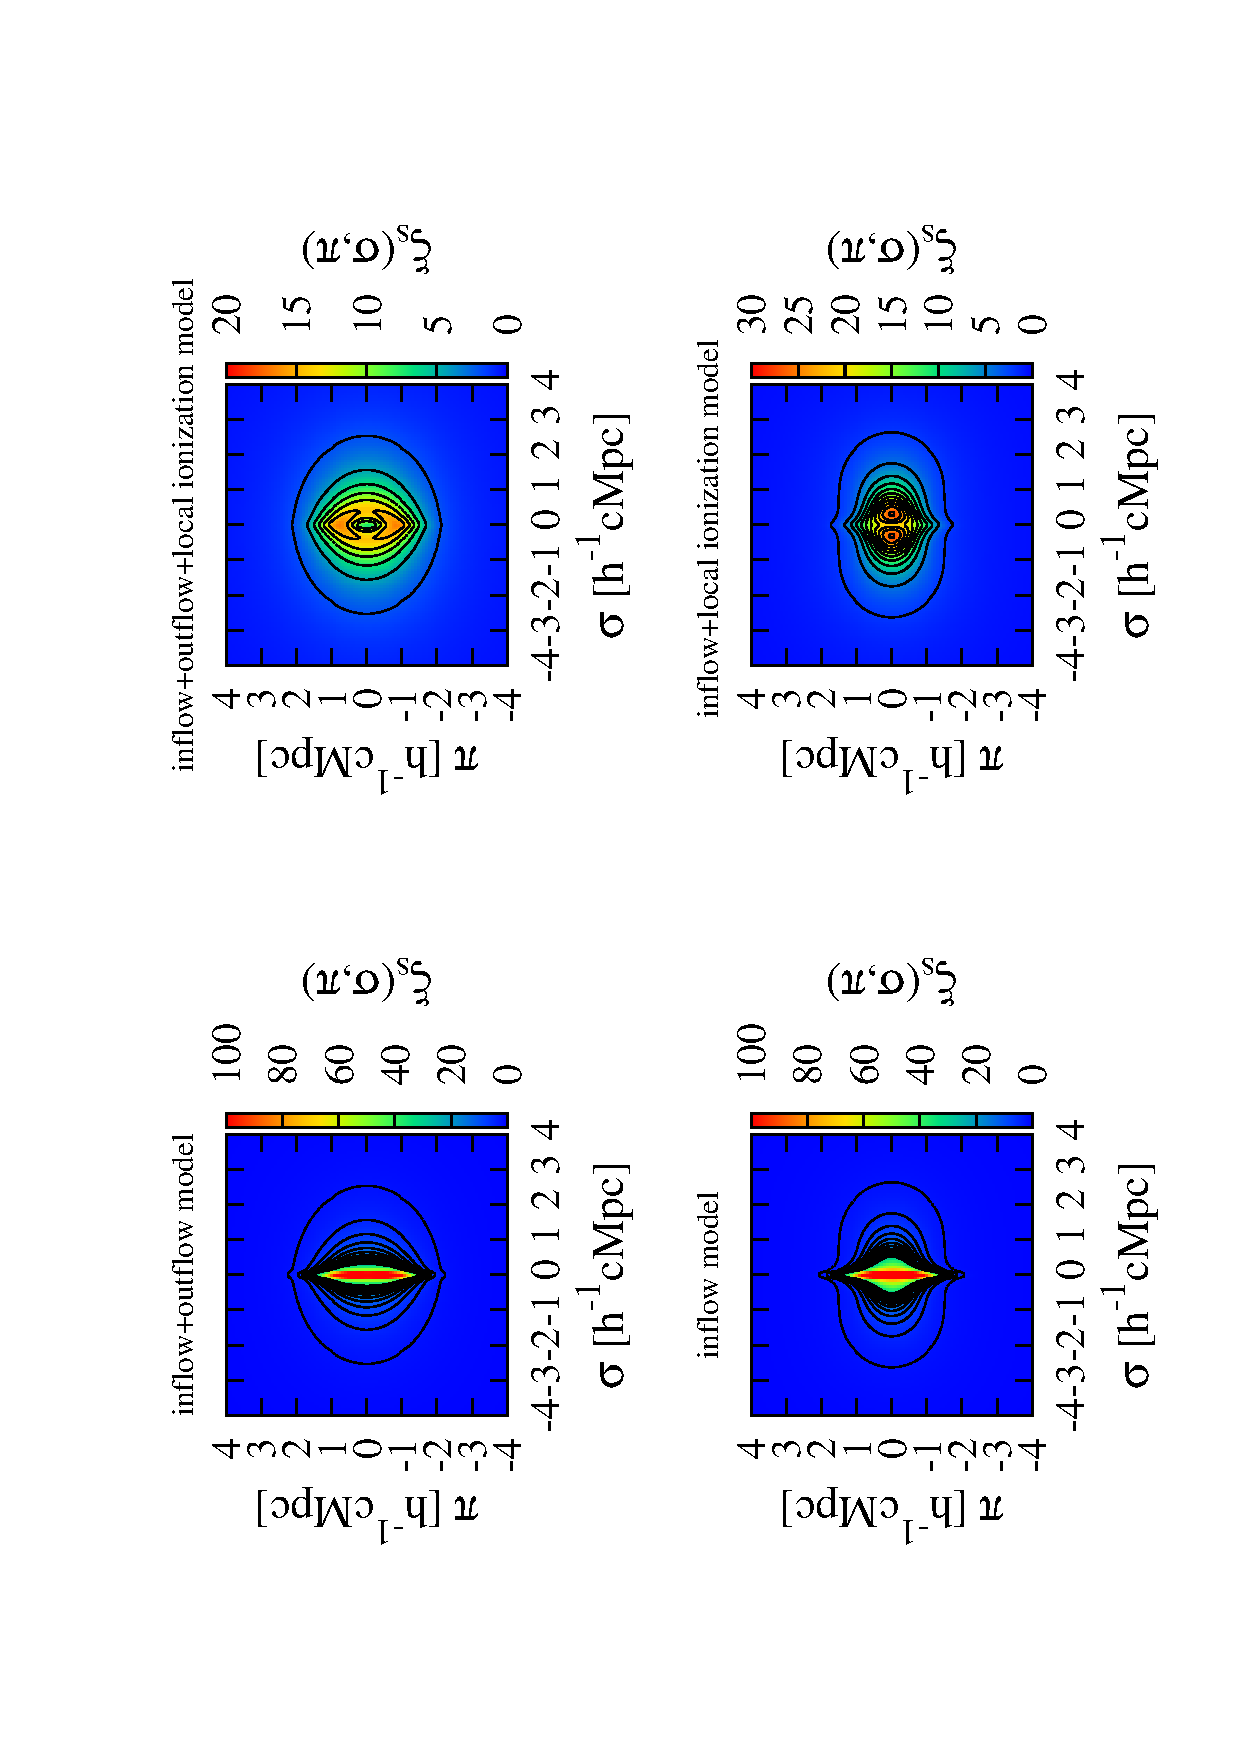
\includegraphics[angle=-90,width=\textwidth]{figure/RSDs.pdf}
  \caption{RSD example}
 \end{center}
\end{figure*}



For linear theory, the correlation function scales as $\propto D(t)^2$,
the pairwise velocity field for unbiased tracer from the linear theory.
\begin{equation}
v_{12}(r)=-\frac{Hf(\Omega_m)}{\pi^2}\int P_L(k)j_1(kr) kdk
\end{equation}
where $f(\Omega)=d\ln D/d\ln a$.


For self-similar clustering,...

\begin{figure}
 \begin{center}
  \includegraphics[angle=0,width=\columnwidth]{figure/v12.pdf}
  \caption{Pairwise velocity field. redo this}
 \end{center}
\end{figure}

\subsubsection{Lagrangian formulation}
The linear theory and the self-similar clustering hypothesis provides
the prototype of real-space 2PCF evolution. The pair conservation law is
more general, which can be applied to outflow. We employ the Lagrangian
picture to illustrate the evolution of 2PCF (Matsubara 2008, Carlson+;
White 2014). 

Lagrangian displacement field $\boldsymbol{\Psi}$ for a fluid element
at $\boldsymbol{q}$ at some initial time,
\begin{equation}
\boldsymbol{r}=\boldsymbol{q}+\boldsymbol{\Psi}(\boldsymbol{q},t)
\end{equation}
The mass conservation implies
\begin{equation}
1+\delta(\boldsymbol{r})=\int d^3q[1+\delta(\boldsymbol{q})]
\delta_D[\boldsymbol{r}-\boldsymbol{q}-\boldsymbol{\Psi}(\boldsymbol{q},t)]
\end{equation}


\section{Theory: The environmental dependence of $\LyA$ visibility}

\subsection{The region of influence}
For both EoR $z>6$ (McQuinn+; Dikjstra+) and the post-reionized universe 
$2<z<6$ (Zheng+; Dijkstra\&Wyithe), the IGM environment influence the
visibility of $\LyA$-emitting galaxies. The degree of the impact depends
on the amount of clustering of gas, velocity field, and photoionization
background in the vicinity of the galaxies. The $\LyA$ radiative transfer
is sensitive to the velocity structure. The gas velocity field is nonlinear
in and out of galactic haloes, but at large enough distance it would 
converge to Hubble flow. The region of influence of $\LyA$ RT is most 
directly characterized in the velocity space. The wing approximation to
the Lorentz profile $\varphi_\nu=\frac{\Lambda/4\pi^2}{(\nu-\nu_\alpha)^2+(\Lambda/4\pi)^2)}
\approx\frac{\Lambda}{4\pi^2(\nu-\nu_\alpha)^2}$ where $\Lambda=6.25\times10^8s^{-1}$ is
the damping coefficient.  The optical depth of 
an absorber of column density $\NHI$ and total (hubble flow plus peculiar)
proper velocity $v_c$ is $\tau_\alpha(\nu_e)=\sigma_\alpha\NHI\varphi_\nu[\nu_e(1-v_c/c)]$
The absorber velocity that gives the optical depth $\tau_\alpha$
against $\LyA$ line emission from galaxies is 
\begin{equation}
v_c(\tau_\alpha)=c\sqrt{\frac{\sigma_\alpha\NHI\Lambda}{4\pi^2\nu_\alpha^2\tau_\alpha}}
=507.3\tau_\alpha^{-1/2}\left(\frac{\NHI}{10^{20}cm^2}\right)^{1/2}\rm{km/s}
\end{equation}
For a strong absorbing cloud to give the optical depth of unity (37\% transmission) 
against the $\LyA$ line emission, the absorbing cloud cannot be 
outflowing relative to the central galaxy more than $\sim500-2800\rm{km/s}$.
This defines the region of influence of $\LyA$ RT in the velocity space.
To translate the region of influence to the real space we need to know the
velocity field around a galaxy. For pure Hubble flow the comoving region of influence
is 
\begin{equation}
D_{\rm{infl}}=\frac{v_c(\tau_\alpha)}{H_0}\frac{1+z}{[\Omega_m(1+z)^3+\Omega_\Lambda]^{1/2}}
\end{equation}
\subsection{Statistical formulation}
The statitical formulation of the $\LyA$ raditive transfer can start
with Paresce, McKee Bowyer 1980. An alternative derivation, which clarifies 
the implicit assumptions and allow generalization, is shown in Appendix.
The critical difference between continuum
RT and line RT is that the former is sentitive to the clustering in real
space whereas the latter is to in \textit{velocity space}.
The probability of an absorbering cloud's velocity within $v$ and $v+dv$
is $p(v)dv$. Then the probability that a line-of-sight of $\LyA$ galaxy to 
the observer does not coincide is $1-p(v)dv$. The fraction of photons absorbed
is $p(v)e^{-\tau(v)}dv$
\begin{equation}
\langle I(v+\Delta v)\rangle=\langle I(v)\rangle
\left\{
(1-p(v)\Delta v)+p(v)e^{-\tau(v)}\Delta v
\right\}
\end{equation}
Forming the differential equation by $d\langle I\rangle/dv\approx
\langle I\rangle[p(v)(1-e^{-\tau(v)})]$, whose solution is
$\langle I\rangle=\langle I\rangle_0e^{-\tau_{\rm{eff}}}$
\begin{equation}
\tau_{\rm{eff}}=\int_{-\infty}^\infty p(v_{12})\left[1-e^{-\tau(v_{12})}\right]dv_{12}
\end{equation}
where $v_{12}^{tot}=aHr_{12}+v_{12}$ is the \textit{total, proper pairwise 
velocity} of absorber and galaxy. By transforming the variables $r_{12}, v_{12}$
into $v_{12}^{tot}$,
\begin{eqnarray}
f(v_{12}^{tot})&=&\iint\delta_D\left[v_{12}^{tot}-(Hr_{12}+v_{12})\right]
f(v_{12},r_{12})dv_{12}dr_{12} \nonumber \\
&=&\int f(v_{12}^{tot}-Hr_{12}|r_{12})f(r_{12})dr_{12}
\end{eqnarray}
where $f(r)dr=\frac{4\pi r^2}{V}(1+\xi(r))dr (NO!)$ 
CORRECT ONE is $f(r)dr=\frac{1}{L}(1+\xi(r))dr$ (pre-factor
dendendence is geometric factor for 1D along a skewer it does not enter!)
is the PDF from the 
real-space clustering of absorber around galaxy.

total velocity $v_\parallel^{tot}=H s_\parallel=H(r_\parallel+v_\parallel/H)$
\begin{equation}
I(s+ds)=I(s)\left\{1-p(s_\parallel,\NHI)ds_\parallel+p(s_\parallel,\NHI)
e^{-\tau(s_\parallel,\NHI)}ds\right\}
\end{equation}


The end result for Gaussian pairwise velocity PDF.

\begin{equation}
\tau_{\rm{eff}}=\int d\NHI\frac{\partial^2\mathcal{N}}{\partial\NHI\partial z}
\left|\frac{dz}{dr}\right|
\int dv f(v_{12})\left[1-e^{-\tau(v_{12},\NHI)}\right]
\end{equation}
\begin{equation}
f(v_{12})=\int \frac{dr}{\sqrt{2\pi\sigma_{12}^2(r)}}
\left(1+\xi(r)\right)
\exp\left[\frac{(v_{12}^{tot}-Hr-\langle v_{12}(r)\rangle)^2}
{2\sigma_{12}^2(r)}\right]
\end{equation}



The end result for Gaussian pairwise velocity PDF.
\begin{equation}
\tau_{\rm{eff}}=\int d\NHI\frac{d\mathcal{N}}{d\NHI}
\int dv f(v_{12})\left[1-e^{-\tau(v_{12},\NHI)}\right]
\end{equation}
\begin{equation}
f(v_{12})=\int \frac{4\pi r^2dr}{\sqrt{2\pi\sigma_{12}^2(r)}V}
\left(1+\xi(r)\right)
\exp\left[\frac{(v_{12}^{tot}-Hr-\langle v_{12}(r)\rangle)^2}
{2\sigma_{12}^2(r)}\right]
\end{equation}


The end result for Gaussian pairwise velocity PDF.
\begin{equation}
\tau_{\rm{eff}}=\int d\NHI\frac{d\mathcal{N}}{d\NHI}
\int dv f(v_{12})\left[1-e^{-\tau(v_{12},\NHI)}\right]
\end{equation}
\begin{equation}
f(v_{12})=\int \frac{4\pi r^2dr}{\sqrt{2\pi\sigma_{12}^2(r)}V}
\left(1+\xi(r)\right)
\exp\left[\frac{(v_{12}^{tot}-Hr-\langle v_{12}(r)\rangle)^2}
{2\sigma_{12}^2(r)}\right]
\end{equation}

For generalization to the anisotropic real-space clustering, e.g.
biconical outflow + two cold streaming model
\begin{equation}
f(v_{12})=\int \frac{d^3r}{\sqrt{2\pi\sigma_{12}^2(\boldsymbol{r})}}
\left(1+\xi(\boldsymbol{r})\right)
\exp\left[\frac{(v_{12}-\langle v_{12}(\boldsymbol{r})\rangle)^2}
{2\sigma_{12}^2(\boldsymbol{r})}\right]
\end{equation}

Pairwise velocity at $\boldsymbol{r}$ is $v_{12}(\boldsymbol{r})$.
$\xi_v(\boldsymbol{r})=\langle v_{12}(\boldsymbol{x})
v_{12}(\boldsymbol{x}+\boldsymbol{r})\rangle$

We can imagine two models, dirac delta PDF $p(v_{12}|r)=\delta_D(v_{12}-aHr)$

\subsection{Caveats}
\subsubsection{Pairwise velocity PDF}
How good is the gaussian approximation to pairwise velocity PDF? The assumption
that the pairwise velocity PDF may introduce systematic bias in analytic model.
Scoccimaro 2004 has studied that the pairwise velocity PDF is in fact highly
non-gaussian with skewness and kurtosis. Tinker 2005? modelled the non-gaussian
pairwise velocity PDF in the HOD framework. Generalisation can also be done
possibly by the cumulant expansion or Edgeworth expansion 
(e.g. Matsubara2008+; Sherrer\&Bertschinger 1991).

Scoccimaro 2004 argued that the direct recontruction of the PDF from 
redshift-space clustering measurement is in general impossible, which
must rely on the assumption of scale-independent PDF or Gaussianity.


The pairwise velocity PDF $p(v_{12})$. Maybe an approach is cumulant
expansion with respect to N-point correlation function derived from 
BBGKY hierarchy. The truncate with 2PCF (see Scherrer \& Bertschinger 1991)? 


\section{Simulation}
\subsection{Cosmological hydrodynamical simulation of the IGM}

\begin{table*}
\centering
\caption{Simulation set up}
\label{table:ramses}
\begin{tabular}{llllllllll}
\hline
name        & Box size $L$       & $N_{\rm{DM}}$ & $N_{\rm{grid}}(base)$ &  $N_{\rm{grid}}(fine)$   & $m_{\rm{DM}}$          &$\Delta L(base)$ & $\Delta L(fine)$  & $z_{ini}$ & $J_{21}, \alpha, z_{reion}$ \\ 
            & [$h^{-1}\rm{cMpc}$] &             &                    &                       & [$h^{-1}\rm{M}_\odot$] &[$h^{-1}\rm{ckpc}$] &             \\
\hline
\multicolumn{2}{l}{\underline{static grid + adiabatic}} \\
L10P256G256R0 &  10              & $256^3$   & $256^3$     &     & $3.57\times10^6$      & 39.1       &        & 276  \\
L20P256G256R0 &  20              & $256^3$   & $256^3$     &    & $2.86\times10^7$      & 78.1        &       & 237   \\
L40P256G256R0 &  40              & $256^3$   & $256^3$     &    & $2.29\times10^8$      & 156.2       &       & 199   \\
L60P256G256R0 &  60              & $256^3$   & $256^3$     &    & $7.72\times10^8$      & 234.4       &       &  178   \\
\multicolumn{2}{l}{\underline{AMR grid + adiabatic}} \\
L40P256G256R2 &  40              & $256^3$   & $256^3$     & $1024^3$   & $2.29\times10^8$      & 156.2      &  39.1      & 199   \\
\multicolumn{2}{l}{\underline{static grid run + UV background}} \\
L40P256G256R0 &  40              & $256^3$   & $256^3$     &    & $2.29\times10^8$      & 156.2       &       & 199   & 1.0, 1.0, 8.5 \\


\hline
\end{tabular}

\end{table*}

We carried out the cosmological hydrodynamical simulation of the IGM using 
AMR hydro/$N$-body code RAMSES (Teyssier 2002). We performed a series of 
adiabatic simulation with varying box size and resolution elements for 
convergence test. 

We adopt the quasi-Lagrangian refinement strategy with refinement criterion 
of 10 particles by which the cell is refined when the number of dark matter 
particle or equivalent gas mass exceeds 10.  

The initial condition is generated with COSMICS package (Bertschinger 1996?). 
The COSMICS package is initialized by setting the initial rms fluctuation 
$\sigma_8(z=z_{ini})=0.03$. Because the resolution of simulations are varying 
the initial redshift is elevated to lower redshift for lower resolution 
simulation. The initial temperature is set as $T=650\rm{K}$.This is compromise 
because the adiabatic simulation does not include Compton heating from CMB and 
cooling. The IGM only be cooled or heated by adiabatic process.

The haloes are identified by HOP algorithm (Eisenstein+; Aubert).

\subsection{Radiative transfer}
We introduce the self-shielded gas by Rhamati+ criterion. The method
is calibrated based on radiative transfer simulation.

\subsection{Synthetic QSO spectra}

\subsection{Synthetic galaxy catalogue}

\section{Comparison between model and simulation}
\subsection{unbiased tracer: gas and dark matter}


\section{survey: mock}

%%%%%%%%%%%%%%%%%%%%%%%%%%%%%%%%%
\bigskip
\section*{acknowledgments}

K.K. thanks to ...

E. Komatsu for Cosmology Routine Library and J. Carlson, B. Reid, M. White
for CLPT and GSRSD code publicly available, from which the analytical
computation routine for this paper is developed.
R. Teyssier and RAMSES development team to make code publicly available
and user friendly.
Some of the calculations in this paper is computed using 
python mpmath library (\citealt{mpmath}).

%%%%%%%%%%%%%%%%%%%%%%%%%%%%%%%%%

\bibliographystyle{mn2e}
\bibliography{Reference}


%%%%%%%%%%%%%%%%%%%%%%%%%%%%%%%%%
\appendix
\section{Statistical formulation of radiative transfer}\label{appendix}
We present the statistical formulation of radiative transfer, which is
the application and the substantial generalization of the ideas appeared 
in Parsce+ 1980, Haardt \& Madau; Zuo; Meiksin\& White; Kakiichi+2012.

The cosmological radiative transfer through the IGM, neglecting the effect
of re-emission and scattering along a line-of-sight is described by
\begin{equation}
\frac{1}{c}\frac{\partial I_{\nu}}{\partial t}
+\boldsymbol{n}\cdot\boldsymbol\nabla I_{\nu}
-\frac{H+\boldsymbol{n\cdot\nabla v\cdot n}}{c}
\nu\frac{\partial I_{\nu}}{\partial \nu}+
3\frac{H}{c}I_{\nu}=-\sigma_\alpha\nHI\varphi_\nu I_{\nu}
\end{equation}
where $I_\nu$ is the specific intensity, $\boldsymbol{v}$ is the peculiar 
velocity, $\boldsymbol{n}$ is the unit direction vector of rays, 
$\sigma_\alpha=0.011\rm cm^2Hz$ is the $\LyA$ cross section,
$\varphi_\nu$ is the line profile of $\LyA$ resonance line. 
$\boldsymbol{n\cdot\nabla v\cdot n}$ term is the Doppler shift effect.
The solution to the cosmological radiative transfer equation is
\begin{equation}
I_\nu=\frac{I_\nu(z_s)}{(1+z_s)^3}e^{-\tau_\alpha(\nu_e,z_s)}
\end{equation}
where the optical depth $\tau_\alpha$ is given by
\begin{equation}
\tau_\alpha(\nu_e,z_s)=\int_0^{z_s}dz'\left|\frac{dl_p}{dz'}\right|
\nHI(z')\varphi_\nu\left[T(z'),\nu_e\left(\frac{1+z'}{1+z_s}\right)
\left(1-\frac{v(z')}{c}\right)\right]
\end{equation}
 
We are interested in the statistical properties of the radiation field $I_\nu$.
The probability distribution function $P(I_\nu)dI_\nu$ provides the probability
that an radiating source is observed  with the specific intensity $I_\nu$.
The averege specific intensity for all the sources 
$\langle I_\nu\rangle=\int I_\nu P(I_\nu)dI_\nu$ corresponds to stacking the 
observed spectra of galaxies or QSOs. 

Suppose a sphere of radius $R$ centred at the obeserver that is sufficiently 
large to contain the source. In the picture that the IGM consists of absorbers
of column density $\NHIi$ and redshift


Suppose a line-of-sight skewer of length $R$.
The optical depth along a line-of-sight is
\begin{equation}
\tau(\nu_e)=\sigma_\alpha\int_0^R dr' \nHI(r')\varphi(r')
=\sigma_\alpha\sum_{i=1}^{\mathcal{N}} \NHIi\varphi(r_i) \Theta(r_i-R)
\end{equation}


\label{lastpage}


\end{document}
